\documentclass[UTF8,a4paper,12pt,fontset=fandol]{ctexart}
\usepackage[left=2.5cm,right=2.5cm,top=2.4cm,bottom=2.4cm]{geometry}
\usepackage{amsmath,amssymb,bm}
\usepackage{booktabs,longtable,tabularx,array,multirow}
\usepackage{graphicx,float,subcaption}
\usepackage{xcolor}
\usepackage{enumitem}
\usepackage{setspace}
\usepackage{fancyhdr}
\usepackage{hyperref}
\usepackage{listings}
\usepackage{caption}
\usepackage{chngcntr}

\hypersetup{colorlinks=true,linkcolor=black,citecolor=black,urlcolor=blue}
\graphicspath{{figures/}}
\captionsetup{font=small,labelsep=quad}
\captionsetup[table]{position=top}
\captionsetup[figure]{position=bottom}
\setstretch{1.22}
\setlength{\parindent}{2em}
\setlength{\parskip}{0pt}
\setlist{nosep,leftmargin=2em}
\pagestyle{fancy}
\fancyhf{}
\cfoot{\thepage}
\renewcommand{\headrulewidth}{0pt}
\renewcommand{\arraystretch}{1.18}
\newcolumntype{Y}{>{\centering\arraybackslash}X}
\newcolumntype{L}{>{\raggedright\arraybackslash}X}
\newcommand{\dif}{\mathop{}\!\mathrm{d}}
\newcommand{\VaR}{\operatorname{VaR}}
\newcommand{\CVaR}{\operatorname{CVaR}}
\newcommand{\logit}{\operatorname{logit}}
\numberwithin{equation}{section}
\counterwithin{figure}{section}
\counterwithin{table}{section}
\renewcommand{\thefigure}{\thesection-\arabic{figure}}
\renewcommand{\thetable}{\thesection-\arabic{table}}

\lstset{
  language=Python,
  basicstyle=\ttfamily\scriptsize,
  keywordstyle=\color{blue!70!black},
  commentstyle=\color{green!45!black},
  stringstyle=\color{orange!70!black},
  numbers=left,
  numberstyle=\tiny\color{gray},
  frame=single,
  breaklines=true,
  showstringspaces=false,
  tabsize=4,
  columns=fullflexible
}

\title{\heiti\bfseries 微网与外部电网电力调控策略优化的的研究}
\author{}
\date{}

\begin{document}
\vspace{-5.5em}
\maketitle
\vspace{-2.2em}

\begin{abstract}
本文针对中小微企业财务信息不充分、信用风险难以准确量化以及突发事件冲击下信贷方案稳定性不足的问题，以企业进销项发票、信誉评级和贷款利率--客户流失率数据为基础，综合运用CRITIC--TOPSIS客观评价、代价敏感Logistic回归、CORAL领域自适应与Monte Carlo情景模拟等方法，构建从信用特征提取、风险量化到授信决策与稳健调整的求解框架，实现对有信贷记录企业的信用风险评价与授信决策、无信贷记录企业的风险迁移，以及突发事件条件下信贷策略稳健调整的求解。

\textbf{针对问题一，}考虑到发票所反映的交易规模、盈利能力、经营稳定性与异常交易特征等信息，以此构建共12项信用特征；采用\textbf{CRITIC--TOPSIS客观评价}确定各项特征权重、计算经营安全度，并以最优融合系数0.90与\textbf{代价敏感Logistic回归}的违约风险加权融合。建立了在年度信贷总额固定、单户额度限制、D级企业禁止放贷约束条件下的\textbf{利率--额度联合离散优化模型}。在5000万元基准预算下共向99家企业授信，预期\textbf{净收益34.10万元}。较好地区分了正常企业与高违约风险企业，并识别出约四分之三的违约企业，具有较好的风险预警能力，可为授信额度与利率的制定提供可靠依据。

\textbf{针对问题二，}考虑无信贷记录企业缺少"是否违约"信息，且有信贷记录企业和无信贷记录企业分布情况不同，以123家有信贷记录企业为源域、302家无信贷记录企业为目标域，引入\textbf{CORAL方法}对齐协方差结构，并通过\textbf{Bootstrap重复拟合}对不确定性较高的企业施加额外惩罚即提升风险评分。完成后两域协方差近似，最终在1亿元信贷总额下向239家企业配置贷款，预期\textbf{净收益163.11万元}。

\textbf{针对问题三，}考虑突发事件对不同行业企业的异质性冲击，结合行业三档收入冲击、企业暴露度与一阶供应链传播构建Monte Carlo情景模型，以均值风险与95\%分位风险的加权值完成稳健配置，并以CVaR检验尾部风险。基于1200个情景调整后共226家企业获贷，平均损失由113.07万元降至96.91万元、95\% CVaR由120.21万元降至102.96万元，较原方案降低14.35\%。

研究结果表明，所建模型能够兼顾多风险识别、收益优化、跨样本迁移与极端风险控制，且对普通数据误差和参数小幅变化具有较强稳定性，可为信息不完全条件下对中小微企业的差异化授信和动态风险管理提供量化依据。

\textbf{关键词：}中小微企业信贷决策；CRITIC--TOPSIS；CORAL迁移学习；离散优化；CVaR
\end{abstract}

\section{问题重述}

\subsection{问题的背景}

中小微企业是吸纳就业、维持产业链活力和促进技术创新的重要主体，但其通常存在经营规模较小、财务制度不完善、抵押资产不足和抗风险能力偏弱等问题。传统银行授信高度依赖资产负债表、抵押物和长期信用记录，难以覆盖具有真实经营活动但缺少标准化信用信息的中小微企业。企业采购和销售形成的发票包含交易金额、发生时间、交易对象和发票状态，能够从侧面反映经营规模、持续性、上下游结构和交易异常，因而可作为信用评价的替代数据，进而决定信贷策略。

银行信贷决策并非简单地选择低风险企业。贷款利率提高可以增加名义利息收入，却会使客户流失概率上升；扩大授信范围有利于完成资金投放，但也可能提高信用损失。因此，需要把信用风险评价、客户流失、贷款利率和额度配置置于同一框架。对于无信贷记录企业，还存在目标样本无是否违约标签和源域、目标域样本分布不同的问题。近年研究表明，借助迁移学习方法能够缓解小微企业信用评分中的高维小样本和冷启动困难\cite{fang2023,suryanto2022}。此外，突发事件会通过行业需求变化和贸易信用网络传播风险\cite{berloco2021}，静态授信方案需要进一步接受风险检验。

\subsection{问题的重新表述}

\textbf{问题1：}（1）依据附件1内有信贷记录企业的相关数据，提取能够反映交易情况的信用特征，建立企业信用风险评价模型；（2）综合考虑贷款利息收入、客户流失和违约损失，制定授信方案；（3）题目未给出第一问信贷总额，故以5000万元作为基准预算，分析授信方案的收益、风险及稳定性。\par


\textbf{问题2：}（1）针对附件2内无信贷记录企业缺少历史违约标签的问题，利用问题1中有标签企业的风险识别规律，建立针对无标签企业的信用风险迁移评价模型；（2）分析源域与目标域企业在特征分布上的差异，处理领域偏移和预测不确定性；（3）在年度信贷总额为1亿元的条件下，结合附件一各评级占比给出各企业的信用等级，决定授信与否、贷款额度和贷款利率，最后评价资金配置的预期收益与风险。


\textbf{问题3：}（1）在问题2授信方案的基础上，考虑突发事件对不同行业企业经营状况的差异化冲击，以及上下游交易关系可能引致的风险传播；（2）构建包含行业收入冲击、企业风险暴露度和一阶供应链传播的随机情景模型，计算企业在不同情景下的违约风险和贷款组合损失；（3）在保持信贷总额为1亿元的前提下，调整企业授信额度与利率，降低组合平均信用损失及极端情景下的尾部风险，并检验调整方案的稳健性。

上述三问依次构成“历史样本风险识别--无标签样本风险迁移--突发情景稳健调整”的递进过程：问题1为后续决策提供风险评价基础模型，问题2将风险评价扩展至无信贷记录企业，问题3进一步优化并检验授信方案在外部冲击下的稳定性。

\section{问题分析}

\subsection{总体思路}

本题是数据驱动的多阶段信用风险决策问题。首先将数百万条发票明细聚合为企业层面的信用特征；然后融合客观综合评价与有监督分类，获得相对违约风险；再将风险、利率、客户流失和损失写入贷款分配策略，形成带业务约束的离散型额度优化；最后通过领域对齐和随机突发风险情景模拟，分别解决无标签迁移和突发事件冲击。

\subsection{问题一分析}

问题一的关键矛盾是多维度的经营信息难以归结为单一的信用风险得分，而风险得分又必须转换为具体的贷款方案。仅使用原信誉评级会忽略发票反映的动态经营状态；仅使用无监督评价则不能学习历史违约规律。为此，先用CRITIC--TOPSIS计算经营安全度，再用类别加权Logistic学习违约规律，通过交叉验证融合二者。随后把客户流失率和违约损失写入风险调整收益函数，枚举利率并配置额度。

\subsection{问题二分析}

问题二内302家无信贷记录企业缺少违约标签，且其特征分布规律与123家有信贷记录企业可能不同，直接套用第一问模型会产生领域偏移。本文以123家企业为源域、302家企业为目标域，采用CORAL对齐协方差结构；再通过Bootstrap重复拟合多次得到风险均值和预测标准差，对不确定性较高的企业实施额外惩罚、提升风险评分，最后沿用第一问的评级尺度和优化后的规则完成1亿元配置。

\subsection{问题三分析}

突发事件具有行业异质性、随机性和传导性。仅按平均冲击调整可能低估小概率重大损失，只按最坏情景决策又可能过度保守。本文依据行业和企业暴露度生成直接冲击，以交易集中度近似一阶供应链传播；通过Monte Carlo形成情景违约概率，使用平均风险与95\%分位风险的加权值配置贷款，再用CVaR衡量最严重5\%情景中的平均损失。

\begin{figure}[H]
\centering
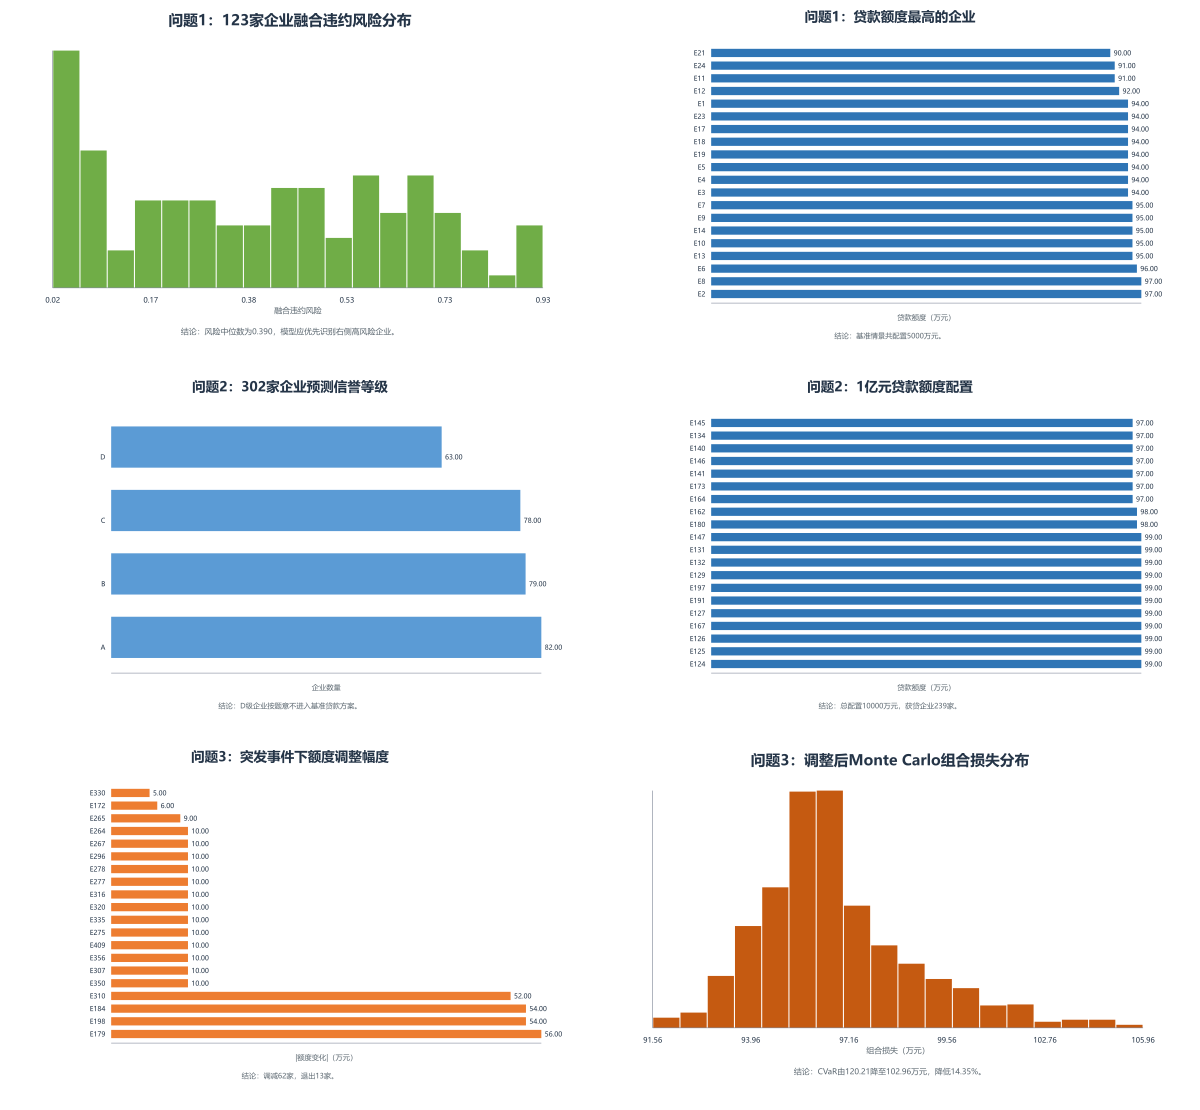
\includegraphics[width=0.95\textwidth]{fig_overview.png}
\caption{三个问题的数据、模型与结果图表总览}
\label{fig:overview}
\end{figure}

\section{模型假设}

\begin{enumerate}
  \item \textbf{发票能大致反映企业经营情况。}将有效进、销项发票视为正常经营记录，作废和红字发票用于反映异常交易，据此提取企业的交易规模、稳定性和异常率等特征。
  \item \textbf{贷款期限按一年计算。}在贷款期内，企业的经营情况和风险水平按已知基准状态处理；突发事件对贷款企业的影响在问题三中单独讨论。
  \item \textbf{企业流失主要受利率和信誉等级影响。}在附件给出的利率范围内，采用相应信誉等级的对应流失率，其他因素暂不单独考虑。
  \item \textbf{两类企业的风险规律基本一致。}有无信贷记录的企业都使用相同的发票特征，因此可借助有记录企业的违约情况来评估无记录企业的风险；样本差异通过CORAL和Bootstrap修正。
  \item \textbf{突发事件的影响主要来自行业和上下游交易。}用企业收入变化表示直接经济冲击，用交易集中度反推上下游对企业的传导影响，据此模拟企业风险和组合损失。
\end{enumerate}

\section{符号说明}

\begin{longtable}{p{0.13\textwidth}p{0.54\textwidth}p{0.16\textwidth}}
\toprule
符号 & 含义 & 单位或范围\\
\midrule
\endfirsthead
\toprule
符号 & 含义 & 单位或范围\\
\midrule
\endhead
$i,j,s$ & 企业、指标和情景编号 & 无量纲\\
$X_{ij},z_{ij}$ & 原始指标及正向化标准指标 & 依指标而定；无量纲\\
$w_j$ & CRITIC客观权重 & $[0,1]$\\
$S_i$ & TOPSIS经营安全度 & $[0,1]$\\
$p_i^L,p_i^T,p_i$ & Logistic风险、TOPSIS风险和融合风险 & $[0,1]$\\
$\theta$ & 风险融合系数 & $[0,1]$\\
$G_i,y_i$ & 企业信誉等级、历史违约状态 & A--D；0或1\\
$x_i,b_i$ & 贷款额度、是否授信变量 & 万元；0或1\\
$r_i,d_i(r_i)$ & 年利率和客户流失率 & $[4\%,15\%]$；$[0,1]$\\
$\eta,\lambda$ & 违约损失率和风险厌恶系数 & 无量纲\\
$B$ & 银行信贷预算 & 万元\\
$\bm C_s,\bm C_t$ & 源域和目标域协方差矩阵 & 无量纲\\
$\bar p_i,\sigma_i,p_i^*$ & Bootstrap平均风险、标准差、修正风险 & $[0,1]$\\
$e_i,h_{is},\rho,\gamma$ & 企业暴露度、情景冲击、传播与放大系数 & 无量纲\\
$L_s(\bm x)$ & 贷款组合在情景$s$中的损失 & 万元\\
\shortstack{$\VaR_\alpha$\\$\CVaR_\alpha$} & 置信水平$\alpha$下的分位损失和尾部均值 & 万元\\
\bottomrule
\end{longtable}

\section{数据预处理与特征构建}

原始发票数据按企业、时间、发票流向和状态进行汇总。首先统一企业编号和日期格式，删除完全重复记录；将有效发票计入正常交易，将作废发票和负数发票分别用于构造异常率数据；对于连续特征采用IQR法检测极端值，并进行上下分位缩尾，以保留异常企业所包含的风险信息而不直接删除样本，防止不合理极端值对特征值的准确性影响。时间序列数据中的少量连续缺失值采用线性预测插入合理值，非时间变量缺失使用同类中位数填补。

最终构建共12项风险特征：有效进项额、有效销项额、净流入代理；进、销项交易对手数；综合作废率、综合负数率；上下游集中度、经营波动率、经营趋势；以及进、销项最大交易对手占比。上述特征分别刻画交易规模、经营活跃度、交易集中度、稳定性和异常交易风险。Logistic和CORAL使用Z-score标准化：
\begin{equation}
z_{ij}=\frac{x_{ij}-\bar x_j}{s_j},
\end{equation}
而TOPSIS使用$[0,1]$正向归一化。所有标准化参数只由相应训练数据计算，以避免验证集信息泄漏。

\section{问题一：融合信用风险与信贷优化}

\subsection{CRITIC--TOPSIS经营评价}

对于正向指标采用
\begin{equation}
z_{ij}=\frac{x_{ij}-\min_i x_{ij}}{\max_i x_{ij}-\min_i x_{ij}},
\end{equation}
负向指标采用其反向形式。第$j$项指标的信息量和权重分别为
\begin{equation}
C_j=\sigma_j\sum_{k=1}^{m}(1-r_{jk}),\qquad
w_j=\frac{C_j}{\sum_{j=1}^{m}C_j}.
\end{equation}
加权矩阵$v_{ij}=w_jz_{ij}$与正、负理想解的距离为
\begin{equation}
D_i^+=\sqrt{\sum_j(v_{ij}-v_j^+)^2},\qquad
D_i^-=\sqrt{\sum_j(v_{ij}-v_j^-)^2},
\end{equation}
经营安全度与评价风险为
\begin{equation}
S_i=\frac{D_i^-}{D_i^++D_i^-},\qquad p_i^T=1-S_i.
\end{equation}

其中，$\sigma_j$为第$j$项指标的样本标准差，$r_{jk}$为第$j$、$k$项指标的Pearson相关系数，$m$为指标数。CRITIC赋权中，进项最大交易对手占比、综合负数率和销项最大交易对手三项占比权重最高，占比的权重分别为0.1166、0.1072和0.0941，表明集中度和异常交易是区分企业间经营安全度差异的重要因素。

\subsection{类别加权Logistic与风险融合}

以$y_i=1$表示历史违约，建立
\begin{equation}
p_i^L=\frac{1}{1+\exp[-(\beta_0+\bm\beta^{\mathrm T}\bm x_i)]}.
\end{equation}
由于违约样本较少，最小化类别加权交叉熵与L2惩罚：
\begin{equation}
\min_{\bm\beta}-\sum_i\omega_i[y_i\ln p_i^L+(1-y_i)\ln(1-p_i^L)]
+\frac{\lambda_r}{2}\|\bm\beta\|_2^2,
\end{equation}
其中，$\omega_i$为按违约类别反比确定的样本权重，$\lambda_r=0.8$为正则化系数，$\bm\beta$为待估回归系数。模型采用IRLS/Newton法迭代，参数最大改变量小于$10^{-7}$时停止。

定义融合风险
\begin{equation}
p_i=\theta p_i^L+(1-\theta)p_i^T,
\end{equation}
并在$[0,1]$内以0.01为步长，选择使五折验证Brier分数最小的$\theta$。得到$\theta^*=0.90$，说明历史违约信息为主、经营评价为辅。

\subsection{利率--额度联合决策}

设客户接受贷款的概率为$a_i(r_i)=1-d_i(r_i)$，其中$d_i(r_i)$表示企业$i$在年利率$r_i$下的流失率；违约损失率$\eta=0.60$表示违约时无法收回的本金比例。每万元贷款的净收益、预期损失和风险调整效用分别为
\begin{align}
e_i(r_i)&=a_i(r_i)[r_i(1-p_i)-\eta p_i],\\
l_i(r_i)&=a_i(r_i)\eta p_i,\\
u_i(r_i)&=e_i(r_i)-\lambda l_i(r_i),\quad \lambda=0.35.
\end{align}
对附件中的利率档枚举，取$r_i^*=\arg\max_r u_i(r)$。额度模型为
\begin{align}
\max\quad &\sum_i x_i u_i(r_i^*),\\
\text{s.t.}\quad&\sum_i x_i=B_1,\\
&10b_i\le x_i\le100b_i,\\
&b_i=0,\quad G_i=D,\\
&x_i\in\mathbb Z_{\ge0},\quad b_i\in\{0,1\}.
\end{align}
本文取$B_1=5000$万元。程序先给可授信企业配置最低额度，再按单位边际效用从高到低、以1万元为步长追加，直至预算耗尽或触及上限。

\subsection{求解结果与分析}

\begin{table}[H]
\centering
\caption{问题一分级风险与贷款配置}
\label{tab:q1}
\begin{tabular}{cccccc}
\toprule
评级 & 企业数 & 平均风险 & 贷款总额/万元 & 平均额度/万元 & 预期净收益/万元\\
\midrule
A & 27 & 0.1950 & 2000 & 74.07 & 24.15\\
B & 38 & 0.3459 & 1658 & 43.63 & 4.79\\
C & 34 & 0.4042 & 1342 & 39.47 & 5.16\\
D & 24 & 0.7051 & 0 & 0 & 0\\
\bottomrule
\end{tabular}
\end{table}

5000万元全部配置给99家A、B、C级企业，D级企业均不授信；组合预期净收益34.10万元，预期损失69.63万元。融合风险均值为0.3990，中位数为0.3895；历史违约组和未违约组的平均风险分别为0.6802和0.3199。风险与额度的相关系数为$-0.9066$，风险与利率的相关系数为0.6347，说明模型实现了高风险低额度及风险溢价定价。

\begin{figure}[H]
\centering
\begin{subfigure}{0.48\textwidth}
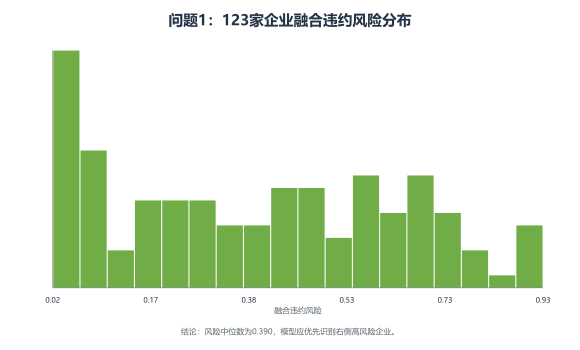
\includegraphics[width=\textwidth]{fig_q1_risk.png}
\caption{融合违约风险分布}
\end{subfigure}\hfill
\begin{subfigure}{0.48\textwidth}
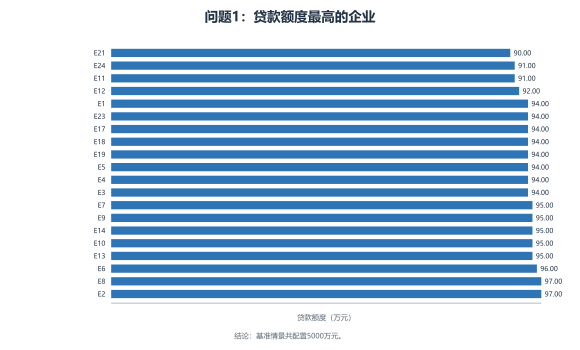
\includegraphics[width=\textwidth]{fig_q1_loan.png}
\caption{额度较高企业的配置}
\end{subfigure}
\caption{问题一风险与信贷配置结果}
\label{fig:q1}
\end{figure}

敏感性分析显示，LGD由0.60降低10\%至0.54时，净收益提高至42.14万元；提高至0.66时，净收益下降至26.39万元。风险厌恶系数在0.315--0.385变化时，净收益仅在33.86--34.27万元间变化。因此方案对实际追偿损失率较敏感，对风险偏好小幅变化较稳定。

\subsection{模型检验}

20次重复五折分层交叉验证结果见表\ref{tab:q1valid}。
\begin{table}[H]
\centering
\caption{问题一重复交叉验证结果}
\label{tab:q1valid}
\begin{tabular}{ccccc}
\toprule
指标 & 均值 & 标准差 & 最小值 & 最大值\\
\midrule
AUC & 0.8030 & 0.0124 & 0.7867 & 0.8291\\
KS & 0.5538 & 0.0369 & 0.4734 & 0.6273\\
Recall & 0.7759 & 0.0306 & 0.7037 & 0.8148\\
Specificity & 0.7281 & 0.0274 & 0.6563 & 0.7813\\
Brier & 0.1751 & 0.0048 & 0.1653 & 0.1821\\
Kappa & 0.3985 & 0.0329 & 0.3432 & 0.4776\\
\bottomrule
\end{tabular}
\end{table}
模型风险等级与人工评级的加权Kappa为0.5091，达到中等一致性。AUC和KS表明模型适合风险排序；但ECE为0.1888，且Brier略高于常数概率基准0.1713，说明具体概率尚需Platt或等距回归校准。加入10\%噪声后，风险排名Spearman仍为0.9906，平均资金重分配比例为2.52\%，模型排序稳定。

\section{问题二：CORAL迁移与一亿元信贷策略}

\subsection{CORAL领域对齐}

记有标签源域为$\mathcal D_s=\{(\bm x_i^s,y_i^s)\}_{i=1}^{123}$，无标签目标域为$\mathcal D_t=\{\bm x_i^t\}_{i=1}^{302}$。分别计算
\begin{equation}
\bm C_s=\operatorname{Cov}(\bm X_s)+\varepsilon\bm I,\qquad
\bm C_t=\operatorname{Cov}(\bm X_t)+\varepsilon\bm I,
\end{equation}
其中$\varepsilon=10^{-4}$。将源域白化后按目标域重新着色：
\begin{equation}
\widetilde{\bm X}_s=(\bm X_s-\bm\mu_s)\bm C_s^{-1/2}\bm C_t^{1/2}+\bm\mu_t.
\end{equation}
于是$\operatorname{Cov}(\widetilde{\bm X}_s)\approx\bm C_t$，使带标签样本的统计结构更接近目标企业。

\subsection{Bootstrap不确定性修正与评级}

对源域进行80次有放回抽样，每次在对齐后的样本上拟合Logistic，得到目标企业预测$\hat p_i^{(b)}$。定义
\begin{equation}
\bar p_i=\frac1{80}\sum_{b=1}^{80}\hat p_i^{(b)},\qquad
\sigma_i=\sqrt{\frac1{79}\sum_{b=1}^{80}(\hat p_i^{(b)}-\bar p_i)^2},
\end{equation}
并构造保守风险
\begin{equation}
p_i^*=\min\{1,\bar p_i+0.20\sigma_i\}.
\end{equation}
按照源域A、B、C、D等级比例，在第一问融合风险上计算分位阈值，并将目标企业由低风险至高风险分级。

将修正风险$p_i^*$代入第一问的收益与损失函数，并重新枚举利率，得到目标域企业的基础单位效用$u_i$。进一步对该效用加入不确定性惩罚：
\begin{equation}
\widetilde u_i=u_i-\eta_u\frac{\sigma_i}{\max_k\sigma_k}\max\{|u_i|,0.01\},\quad \eta_u=0.20.
\end{equation}
个体额度上限为
\begin{equation}
\bar x_i=\left\lfloor10+90(1-p_i^*)^{1.4}
\left(1-0.45\frac{\sigma_i}{\max_k\sigma_k}\right)\right\rfloor.
\end{equation}
在$\sum_i x_i=10000$、$10b_i\le x_i\le\bar x_ib_i$和D级禁贷约束下最大化$\sum_i x_i\widetilde u_i$。

\subsection{求解结果与分析}

\begin{table}[H]
\centering
\caption{问题二迁移评级与贷款配置}
\label{tab:q2}
\begin{tabular}{ccccccc}
\toprule
等级 & 企业数 & 平均风险 & 贷款总额 & 平均额度 & 平均利率 & 预期净收益\\
 & & & /万元 & /万元 & /\% & /万元\\
\midrule
A & 82 & 0.0407 & 7448 & 90.83 & 8.49 & 186.61\\
B & 79 & 0.2816 & 1772 & 22.43 & 14.98 & $-1.34$\\
C & 78 & 0.5614 & 780 & 10.00 & 15.00 & $-22.16$\\
D & 63 & 0.8139 & 0 & 0 & -- & 0\\
\bottomrule
\end{tabular}
\end{table}

共239家企业获得贷款，63家D级企业不授信，1亿元全部配置；预期净收益163.11万元，预期损失103.84万元。A类企业占预算74.48\%，资金显著向低风险企业集中。修正风险与额度的相关系数为$-0.8509$，预测不确定性与额度的相关系数为$-0.6895$，说明模型同时惩罚高风险和高不确定性。

B、C类合计净收益为负，源于题目“总额为1亿元”的强等式解释：A类风险容量不足以单独承接全部预算，剩余资金被配置给相对次优企业。实际应用可增加$\sum_i x_i\le10000$的对照情景，并为未投放资金设置机会收益。

\begin{figure}[H]
\centering
\begin{subfigure}{0.48\textwidth}
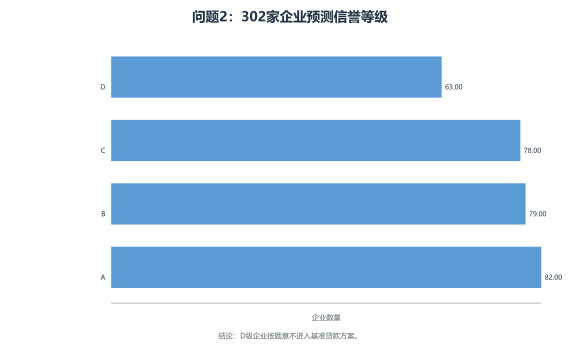
\includegraphics[width=\textwidth]{fig_q2_grade.png}
\caption{302家企业预测等级}
\end{subfigure}\hfill
\begin{subfigure}{0.48\textwidth}
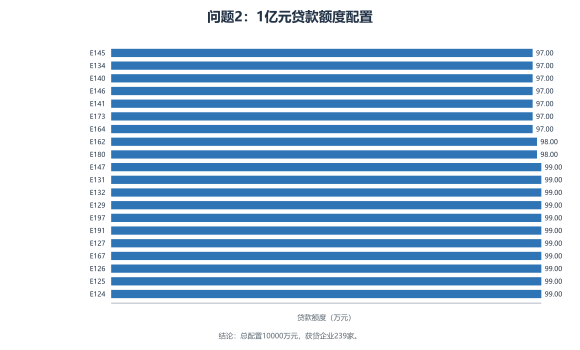
\includegraphics[width=\textwidth]{fig_q2_loan.png}
\caption{一亿元额度配置}
\end{subfigure}
\caption{问题二迁移评级与信贷结果}
\label{fig:q2}
\end{figure}

\subsection{模型检验}

以Frobenius范数衡量协方差差异：
\begin{equation}
D_C=\|\bm C_s-\bm C_t\|_F.
\end{equation}
对齐前$D_C=3.8674$，对齐后为0.000362，改善99.99\%；平均标准化均值差异由0.1144降至接近0。该结果证明统计结构对齐，而非目标域预测准确率达到99.99\%，真实精度仍需后续违约标签验证。

10\%噪声下，风险排序Spearman为0.9918，等级一致率91.67\%，获贷集合Jaccard为0.9552，平均资金重分配比例2.82\%。不确定性系数从0.18增至0.22时，获贷企业从241家降至238家，净收益从163.91万元降至161.67万元，配置结构未发生剧烈改变。

\section{问题三：突发事件下的稳健信贷调整}

\subsection{行业冲击与企业暴露度}

依据企业名称将企业识别为制造业、批发零售、住宿餐饮及生活服务、建筑房地产、交通物流、科技信息服务、医疗健康和其他行业。定义暴露度
\begin{equation}
e_i=0.45c_i+0.35v_i+0.20a_i,
\end{equation}
其中$c_i$为上下游集中度，$v_i$为标准化经营波动率，$a_i$为作废率与负数率之和。集中度高、波动大、异常发票多的企业受到冲击时更脆弱。

各行业设置轻、中、重三档收入冲击中心，发生概率分别为0.15、0.70和0.15；其中$\delta_g<0$表示行业$g$的收入下降比例。在档位中心加入标准差为$\max\{0.18|\delta_g|,0.015\}$的正态扰动，得到情景冲击$\widetilde\delta_{g(i),s}$。企业直接风险冲击为
\begin{equation}
h_{is}^{D}=-\widetilde\delta_{g(i),s}(0.45+0.55e_i).
\end{equation}
以行业平均冲击和集中度构造一阶传播：
\begin{equation}
h_{is}^{P}=\rho c_i\bar h_{g(i),s}^{D},\qquad \rho=0.30,
\end{equation}
总冲击$h_{is}=\operatorname{clip}(h_{is}^{D}+h_{is}^{P},-0.20,1.00)$。

\subsection{情景违约概率与稳健风险}

冲击作用于Logit空间：
\begin{equation}
p_{is}^{\mathrm{shock}}=
\frac{1}{1+\exp[-(\logit(p_i)+\gamma h_{is})]},\qquad \gamma=1.15.
\end{equation}
由$S=1200$个情景计算企业平均风险$\bar p_i^{\,s}=S^{-1}\sum_{s=1}^{S}p_{is}^{\mathrm{shock}}$和95\%分位风险$p_{i,0.95}^{\,s}$，构造
\begin{equation}
p_i^R=0.55\bar p_i^{\,s}+0.45p_{i,0.95}^{\,s}.
\end{equation}
再以$p_i^R$替代基础风险、将风险厌恶系数提高至0.55，并重新枚举利率后沿用第二问的额度优化规则。

情景$s$中的组合损失为
\begin{equation}
L_s(\bm x)=\sum_i x_i[1-d_i(r_i)]p_{is}^{\mathrm{shock}}\eta.
\end{equation}
尾部风险采用
\begin{equation}
\CVaR_\alpha=\min_\tau\left\{\tau+\frac{1}{(1-\alpha)S}
\sum_{s=1}^S\max[L_s(\bm x)-\tau,0]\right\},\quad\alpha=0.95.
\end{equation}
程序使用均值--P95风险作为易求解的稳健代理进行配置，再使用上述CVaR对调整方案进行外部验收。

\subsection{求解结果与分析}

调整后仍投放10000万元，共226家企业获贷。相较问题二，6家调增、62家调减、13家退出。表\ref{tab:q3}表明平均损失和尾部损失同步下降。

\begin{table}[H]
\centering
\caption{突发情景下原方案与调整方案比较}
\label{tab:q3}
\begin{tabular}{cccc}
\toprule
指标 & 原方案/万元 & 调整方案/万元 & 改善幅度\\
\midrule
平均损失 & 113.07 & 96.91 & 14.29\%\\
$\VaR_{0.95}$ & -- & 101.44 & --\\
$\CVaR_{0.95}$ & 120.21 & 102.96 & 14.35\%\\
\bottomrule
\end{tabular}
\end{table}

企业平均冲击为0.1015，平均风险增量为0.0184；冲击强度与风险增量相关系数为0.6200，企业暴露度与风险增量相关系数为0.4046。住宿餐饮及生活服务业平均冲击最大，医疗健康行业在部分情景中受益。行业内部仍存在明显异质性，因而模型进行企业级而非简单行业级增减。

\begin{figure}[H]
\centering
\begin{subfigure}{0.48\textwidth}
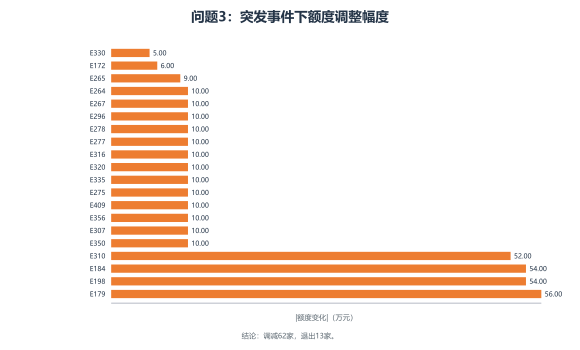
\includegraphics[width=\textwidth]{fig_q3_adjust.png}
\caption{企业额度调整幅度}
\end{subfigure}\hfill
\begin{subfigure}{0.48\textwidth}
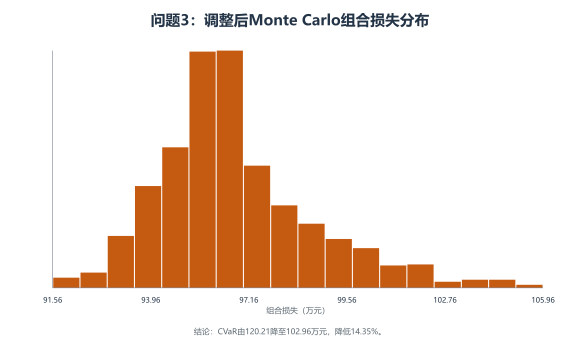
\includegraphics[width=\textwidth]{fig_q3_loss.png}
\caption{调整后情景损失分布}
\end{subfigure}
\caption{问题三额度调整与组合损失}
\label{fig:q3}
\end{figure}

\subsection{模型检验}

随着情景数由200增加至1200，CVaR依次为103.255、103.188、103.326、103.161、103.062和102.956万元，相对最终值最大偏差不超过0.36\%，表明1200个情景已基本收敛。

传播系数$\rho$上下变化10\%时，获贷企业数保持226家，CVaR变化约0.15\%；风险放大系数$\gamma$上下变化10\%时，获贷企业数为225--228家，CVaR变化约1.2\%。10\%输入噪声下，风险排序Spearman为0.9889，等级一致率91.32\%，平均资金重分配比例2.35\%，CVaR最大相对变化2.40\%。模型具有较强抗干扰能力。

\section{模型综合评价}

\subsection{模型优点}

\begin{enumerate}
  \item \textbf{评价与预测融合。}CRITIC--TOPSIS补充经营解释，Logistic利用违约标签，平均AUC达到0.8030、KS达到0.5538，兼顾可解释性和排序能力。
  \item \textbf{从评分直接落地到决策。}利率、流失率、违约损失和额度在同一效用框架内求解，三问均严格满足预算、10--100万元额度和D级禁贷约束。
  \item \textbf{能够处理无标签冷启动。}CORAL使协方差差异降低99.99\%，Bootstrap又显式惩罚不确定性；10\%噪声下目标域风险排序相关仍为0.9918。
  \item \textbf{关注极端损失。}稳健调整使平均损失下降14.29\%、CVaR下降14.35\%，且情景收敛偏差小于0.36\%。
  \item \textbf{易复现和扩展。}核心运算为矩阵分解、重复拟合和排序，复杂度约为$O(nm^2+m^3+Sn+n\log n)$；本题$m=12,n\le302,S=1200$，无需商业软件即可完成。
\end{enumerate}

\subsection{模型不足与改进}

\begin{enumerate}
  \item 123家源域样本偏少，概率校准不足；ECE为0.1888，Brier未显著优于常数概率基准。未来应增加跨年度数据并进行Platt或等距校准。
  \item 目标域没有真实违约标签，CORAL只能证明统计结构对齐，不能替代外部精度检验；可采用类别条件CORAL、MMD和高置信伪标签，并用后续违约数据验证。
  \item 行业冲击和传播参数包含情景假设，且供应链只采用一阶代理；可引入真实行业产出、停工率和交易网络，并直接求解CVaR混合整数模型。对1亿元预算也应同时考察“必须全部投放”和“允许保留流动性”两种政策。
\end{enumerate}

\section{结论}

本文围绕中小微企业信贷风险评价、无标签企业风险迁移和突发事件稳健调整建立了一套递进式模型。第一问通过CRITIC--TOPSIS与代价敏感Logistic融合，把发票经营行为与历史违约信息结合；第二问使用CORAL与Bootstrap将风险知识迁移至无信贷记录企业；第三问利用行业冲击、暴露度和一阶传播构建随机情景，并以CVaR检验尾部损失。

结果显示，模型能够有效区分企业风险并形成满足业务约束的差异化授信方案。领域迁移显著缩小了源、目标样本的统计差异，稳健调整在总额不变的情况下明显降低极端情景损失。噪声试验、敏感性分析和收敛检验进一步表明，主要结论对普通数据误差和参数小幅变化较稳定。该框架可推广到供应链金融、小微企业保险定价和无抵押经营贷等相似场景。

\begin{thebibliography}{99}
\bibitem{fang2023} 方匡南, 李晶茂, 范新妍, 等. 基于多源域知识迁移学习的小微企业信用评分[J]. 系统工程理论与实践, 2023, 43(5): 1320--1332. DOI: 10.12011/SETP2021-2526.
\bibitem{xie2021} 解维敏, 吴浩, 冯彦杰. 数字金融是否缓解了民营企业融资约束?[J]. 系统工程理论与实践, 2021, 41(12): 3129--3146. DOI: 10.12011/SETP2021-1522.
\bibitem{zeng2022} 曾燕, 杨雅婷, 徐凤敏, 等. 消费金融研究综述[J]. 系统工程理论与实践, 2022, 42(1): 84--109.
\bibitem{suryanto2022} Suryanto H, Mahidadia A, Bain M, et al. Credit risk modeling using transfer learning and domain adaptation[J]. Frontiers in Artificial Intelligence, 2022, 5: 868232. DOI: 10.3389/frai.2022.868232.
\bibitem{berloco2021} Berloco C, De Francisci Morales G, Frassineti D, et al. Predicting corporate credit risk: Network contagion via trade credit[J]. PLOS ONE, 2021, 16(4): e0250115. DOI: 10.1371/journal.pone.0250115.
\bibitem{arcuri2023} Arcuri M C, Gandolfi G, Laurini F. Robust portfolio optimization for banking foundations: A CVaR approach for asset allocation with mandatory constraints[J]. Central European Journal of Operations Research, 2023, 31(2): 557--581. DOI: 10.1007/s10100-022-00821-5.
\bibitem{pinar2022} Benati S, Conde E. A relative robust approach on expected returns with bounded CVaR for portfolio selection[J]. European Journal of Operational Research, 2022, 296(1): 332--352. DOI: 10.1016/j.ejor.2021.04.038.
\bibitem{liao2022} Liu W, Yang L, Yu B. Kernel density estimation based distributionally robust mean-CVaR portfolio optimization[J]. Journal of Global Optimization, 2022, 84(4): 1053--1077. DOI: 10.1007/s10898-022-01177-5.
\bibitem{geron2022} G\'eron A. Hands-On Machine Learning with Scikit-Learn, Keras, and TensorFlow: Concepts, Tools, and Techniques to Build Intelligent Systems[M]. 3rd ed. Sebastopol: O'Reilly Media, 2022.
\end{thebibliography}

\appendix
\section{程序环境与运行方法}

程序使用Python 3.14.5，NumPy 2.5.1，Pandas 3.0.5和OpenPyXL 3.1.5。安装与运行命令为：
\begin{lstlisting}[language=bash,numbers=none]
pip install numpy pandas openpyxl
python code/model_solver.py
python code/result_analysis.py
python code/model_validation.py
\end{lstlisting}
完整程序随Overleaf工程存放于\texttt{code/}目录。\texttt{model\_solver.py}完成三个问题的建模与求解；\texttt{result\_analysis.py}完成描述统计和敏感性分析；\texttt{model\_validation.py}完成交叉验证、领域检验、收敛和噪声鲁棒性分析。为控制论文页数，以下列出关键程序片段，完整源代码作为电子附录提交。

\begin{lstlisting}[caption={风险融合与迁移预测核心代码}]
# Q1: fuse supervised risk and TOPSIS risk
theta_grid = np.linspace(0, 1, 101)
briers = [np.mean((t * cv_pred + (1-t) * topsis_risk-y)**2)
          for t in theta_grid]
theta = theta_grid[np.argmin(briers)]
risk1 = theta * logit_prob + (1-theta) * topsis_risk

# Q2: CORAL alignment and uncertainty correction
Xs_aligned = (Xs-ms) @ matrix_power(Cs, -0.5) \
             @ matrix_power(Ct, 0.5) + mt
risk_mean = boot_pred.mean(axis=0)
risk_std = boot_pred.std(axis=0, ddof=1)
risk2 = np.clip(risk_mean + 0.20*risk_std, 0.001, 0.999)
\end{lstlisting}

\begin{lstlisting}[caption={情景风险与CVaR核心代码}]
stress_prob = sigmoid(logit_base[None, :] + gamma * shocks)
robust_risk = np.clip(0.55 * stress_prob.mean(axis=0)
                      + 0.45 * np.quantile(stress_prob, 0.95, axis=0),
                      0.001, 0.999)
scenario_loss = np.sum(loan[None, :] * accept[None, :]
                       * stress_prob * lgd, axis=1)
var95 = np.quantile(scenario_loss, 0.95)
cvar95 = scenario_loss[scenario_loss >= var95].mean()
\end{lstlisting}

\section{中间结果与数据文件}

CRITIC权重向量按12项指标顺序为
\begin{equation}
\begin{aligned}
\bm w=(&0.07981,0.07289,0.07233,0.06559,0.06524,0.08112,\\
       &0.10719,0.08038,0.08700,0.07774,0.11659,0.09410),
\end{aligned}
\end{equation}
且$\sum_jw_j=1$。CORAL对齐前后的协方差距离为3.867436和0.000362。三个问题的总额差、低于10万元户数、超过100万元户数和D级贷款总额均为0。

处理后的特征库及完整结果位于\texttt{data/}目录，包括：
\begin{enumerate}
  \item \texttt{2020C\_数据预处理与特征库.xlsx}：原始特征、缩尾特征、标准化特征和处理记录；
  \item \texttt{问题1\_风险与信贷策略.csv}：123家企业风险、额度、利率和收益；
  \item \texttt{问题2\_风险迁移与1亿元策略.csv}：302家企业迁移风险、评级和策略；
  \item \texttt{问题3\_突发事件稳健调整策略.csv}：行业冲击、稳健风险及额度变化；
  \item \texttt{问题3\_MonteCarlo情景损失.csv}：1200个情景的原方案和调整方案损失；
  \item \texttt{输入噪声鲁棒性汇总.csv}和\texttt{参数敏感性分析.csv}。
\end{enumerate}

\section{补充检验表}

\begin{table}[H]
\centering
\caption{10\%输入噪声下的鲁棒性结果}
\begin{tabular}{ccccc}
\toprule
问题 & 排名Spearman & 等级一致率 & 获贷Jaccard & 平均重分配比例\\
\midrule
问题一 & 0.9906 & -- & 1.0000 & 2.52\%\\
问题二 & 0.9918 & 91.67\% & 0.9552 & 2.82\%\\
问题三 & 0.9889 & 91.32\% & 0.9284 & 2.35\%\\
\bottomrule
\end{tabular}
\end{table}

\begin{table}[H]
\centering
\caption{Monte Carlo样本量收敛检验}
\begin{tabular}{ccccc}
\toprule
情景数 & 平均损失/万元 & VaR/万元 & CVaR/万元 & CVaR相对偏差\\
\midrule
200 & 97.072 & 101.459 & 103.255 & 0.291\%\\
400 & 97.024 & 101.794 & 103.188 & 0.226\%\\
600 & 96.931 & 101.911 & 103.326 & 0.359\%\\
800 & 96.902 & 101.722 & 103.161 & 0.199\%\\
1000 & 96.918 & 101.540 & 103.062 & 0.103\%\\
1200 & 96.911 & 101.445 & 102.956 & 0\\
\bottomrule
\end{tabular}
\end{table}

\end{document}